% !TeX program = xelatex
% !BIB program = biber
\documentclass[light]{lutbeamer}

\usepackage{pgfpages}
\usepackage{ragged2e}
\usepackage{booktabs}
\usepackage{amssymb}
\usepackage{fontawesome5}
\usepackage{tikz}
\usepackage{pgfplots}
\pgfplotsset{compat=1.18}
\addbibresource{references.bib}

% ===================================================================
% METADATA (DERS KİMLİK BİLGİLERİ)
% ===================================================================
\setdepartment{OSTİM TEKNİK ÜNİVERSİTESİ}
\institute{}
\author[Mühendislik Fakültesi]{\\
Prof.~Dr.~Yalçın ATA \\
Prof.~Dr.~Arif DEMİR \\
Dr.~Öğr.~Üyesi~Muhammed ELMNEFİ \\
Dr.~Öğr.~Üyesi~Haydar KILIÇ \\
Dr.~Öğr.~Üyesi~Emel GÜVEN \\
Dr.~Öğr.~Üyesi~Ufuk ASIL \\
Öğr.~Gör.~Sema ÇİFTÇİ
}
\title{MATH 204 -- Olasılık ve İstatistik}
\subtitle{Hafta 3: Bağımsızlık, Tam Bağımsızlık, Toplam Olasılık, Bayes Teoremi}
\date{2025--2026 Bahar Dönemi}

% ===================================================================
% OTOMATİK İÇİNDEKİLER (SUNUM AKIŞI)
% ===================================================================
\setcounter{tocdepth}{2}

\AtBeginSection[]{
  \begin{frame}{Sunum Akışı}
    \scriptsize
    \begin{columns}[T]
    \begin{column}{0.48\textwidth}
        \tableofcontents[sections={1-4}, currentsection]
      \end{column}
      \begin{column}{0.48\textwidth}
        \tableofcontents[sections={5-10}, currentsection]
      \end{column}
    \end{columns}
  \end{frame}
}

\begin{document}

\setbeamertemplate{navigation symbols}{}
\setbeamertemplate{footline}{
  \begin{beamercolorbox}[wd=\paperwidth, ht=10pt, dp=1pt]{footline}
    \usebeamerfont{footline}
    \begin{tikzpicture}[remember picture,overlay]
      \node[anchor=south west, xshift=10mm, yshift=.4mm]
      at (current page.south west)
      {\insertshortauthor,~\department};
    \end{tikzpicture}
    \begin{tikzpicture}[remember picture,overlay]
      \node[anchor=south east, xshift=-5mm, yshift=0.5mm]
      at (current page.south east)
      {\insertframenumber \,/\, \inserttotalframenumber};
    \end{tikzpicture}
  \end{beamercolorbox}
}

% ===================================================================
% KAPAK SLAYTLARI
% ===================================================================

% Görsel Tam Kapak (Logosuz)
\begin{frame}<article:0>[plain,noframenumbering]
    \begin{tikzpicture}[remember picture,overlay]
        \node[anchor=center, at=(current page.center), inner sep=0pt] {
            \includegraphics[width=\paperwidth, height=\paperheight]{logos/background_figure.jpg}
        };
    \end{tikzpicture}
\end{frame}

% Resmi Başlık Sayfası (kapak için özel alt bilgi)
{
  \setbeamertemplate{footline}{
    \begin{beamercolorbox}[wd=\paperwidth, ht=10pt, dp=1pt]{footline}
      \usebeamerfont{footline}
      \begin{tikzpicture}[remember picture,overlay]
        \node[anchor=south west, xshift=10mm, yshift=.4mm, align=left]
        at (current page.south west)
        {\tiny Bu şablon OTÜ Yazılım Mühendisliği tarafından hazırlanmış olup \href{https://github.com/ufukasia/Ostim-Teknik--niversitesi-Yaz-l-m-M-hendisli-i---Lutbeamer-egitim-i-eri-i-haz-rlama-}{buradan} güncel haline ulaşabilirsiniz.};
      \end{tikzpicture}
      \begin{tikzpicture}[remember picture,overlay]
        \node[anchor=south east, xshift=-5mm, yshift=0.5mm]
        at (current page.south east)
        {\insertframenumber \,/\, \inserttotalframenumber};
      \end{tikzpicture}
    \end{beamercolorbox}
  }
  \maketitle{}
}

% GENEL İÇERİK HARİTASI
\begin{frame}{İçindekiler}
  \scriptsize
  \begin{columns}[T]
    \begin{column}{0.48\textwidth}
      \tableofcontents[sections={1-4}]
    \end{column}
    \begin{column}{0.48\textwidth}
      \tableofcontents[sections={5-10}]
    \end{column}
  \end{columns}
\end{frame}

% ===================================================================
% ICERIK: HAFTA 3 - OLASILIK
% ===================================================================


\section{Hafta 2'den Köprü}
\subsection{Hatırlatma ve Öğrenme Planı}

\begin{frame}{Hafta 2'den Ne Getiriyoruz?}
    \begin{block}{Temel Hatırlatma}
        Bu haftanın tamamı, geçen haftaki iki fikrin üstüne kurulur:
        \[
        P(A|B)=\frac{P(A\cap B)}{P(B)}, \qquad
        P(A\cap B)=P(A)P(B|A).
        \]
    \end{block}

    \begin{itemize}
        \item Koşullu olasılık: ``evreni daraltıp'' hesap yapmak.
        \item Çarpım kuralı: birlikte olma olasılığını sıralı düşünmek.
        \item Bu hafta: \textbf{Bağımsızlık}, \textbf{Tam Bağımsızlık}, \textbf{Toplam Olasılık}, \textbf{Bayes}.
    \end{itemize}
\end{frame}

\subsection{Motivasyon: Tek Kanıtla İnanç Güncelleme}

\begin{frame}{Motivasyon: ``Gülümsedi'' \texorpdfstring{$\Rightarrow$}{->} ``Seviyor'' mu?}
    \footnotesize
    \begin{columns}[T]
        \begin{column}{0.4\textwidth}
            \begin{block}{Hipotez ve kanıt}
                \begin{itemize}
                    \item $A$: ``Karşı taraf beni seviyor''
                    \item $B$: ``Bana gülümsedi''
                \end{itemize}
            \end{block}

            \begin{alertblock}{Dikkat: En sık yanılgı}
                \[
                P(A\mid B)\ \text{(gülümsediyse seviyor mu?)}
                \]
                \[
                \neq\ P(B\mid A)\ \text{(seviyorsa gülümser mi?)}
                \]
            \end{alertblock}

            \begin{block}{Bayes kuralı}
                \[
                P(A\mid B)=\frac{P(B\mid A)\,P(A)}{P(B)}.
                \]
            \end{block}

        \end{column}

        \begin{column}{0.55\textwidth}
            \centering
            \includegraphics[width=1\textwidth,height=1\textheight,keepaspectratio]{figures/baes.png}
            \vspace{0.15cm}

            \tiny
            \vspace{-1cm}
            \textit{İkonik mesaj: Kanıtı (\(B\)) görünce hipotezi (\(A\)) güncelle.}
        \end{column}
    \end{columns}
\end{frame}

\begin{frame}{Sayısal Mini Örnek: \texorpdfstring{$P(B)$}{P(B)} neden kritik?}
    \small
    \begin{columns}[T]
        \begin{column}{0.58\textwidth}
            \begin{block}{Makul varsayımlar (örnek amaçlı)}
                \begin{itemize}
                    \item Önsel: $P(A)=0.10$ \hfill (\%10: başlangıç inancı)
                    \item Kanıt gücü: $P(B\mid A)=0.70$ \hfill (seviyorsa gülümsemesi)
                    \item Alternatif: $P(B\mid A')=0.30$ \hfill (sevmese de gülümseyebilir)
                \end{itemize}
            \end{block}

            \begin{block}{Önce payda: Toplam Olasılık}
                \[
                P(B)=P(B\mid A)P(A)+P(B\mid A')P(A').
                \]
            \end{block}

            \begin{itemize}
                \item Bayes hesabında payda, kanıtın ``genel sıklığını'' taşır.
                \item Kanıt toplumda çok sık görülüyorsa ayırt edicilik azalır.
            \end{itemize}
        \end{column}

        \begin{column}{0.38\textwidth}
            \begin{block}{Hesap}
                \footnotesize
                \[
                P(B)=0.70(0.10)+0.30(0.90)=0.34
                \]
                \[
                P(A\mid B)=\frac{0.70(0.10)}{0.34}=\frac{0.07}{0.34}\approx 0.206
                \]
            \end{block}

            \begin{alertblock}{Sonuç}
                Gülümsedi diye olasılık \%10'dan \textbf{\%20.6'ya} çıkar;
                ama \textbf{\%70 olmaz}.
            \end{alertblock}

            \tiny
            \textit{Tek kanıt, inancı günceller; doğrudan ``kesinlik'' üretmez.}
        \end{column}
    \end{columns}
\end{frame}

\begin{frame}{Bu ikonik örnekten Teoreme: Haftanın Zinciri}
    \footnotesize
    \begin{columns}[T]
        \begin{column}{0.58\textwidth}
            \begin{block}{Bayes'in ezbersiz okunuşu}
                \[
                P(A\mid B)=\frac{P(A\cap B)}{P(B)}
                \]
                \begin{itemize}
                    \item Pay: ``Hem $A$ hem $B$'' (ilgili yol)
                    \item Payda: ``$B$'yi üreten tüm yollar'' (toplam)
                \end{itemize}
            \end{block}

            \begin{block}{Neden bu hafta birlikte?}
                \[
                \begin{aligned}
                    \text{Çarpım:}\quad & P(A\cap B)=P(A)P(B\mid A) \\
                    \text{Toplam:}\quad & P(B)=P(B\mid A)P(A)+P(B\mid A')P(A') \\
                    \text{Bayes:}\quad & P(A\mid B)=\frac{P(A\cap B)}{P(B)}
                \end{aligned}
                \]
            \end{block}
        \end{column}

        \begin{column}{0.38\textwidth}
            \begin{alertblock}{Ders mesajı (tek cümle)}
                Bir kanıtı gördüğünüzde önce yönü doğru seçin: \\
                \(P(A\mid B)\) mi, yoksa \(P(B\mid A)\) mı?
                Sonra paydada \textbf{tüm yolları} sayın.
            \end{alertblock}

        \end{column}
    \end{columns}
\end{frame}

\begin{frame}{Bu Haftanın Öğrenme Hedefleri}
    \begin{enumerate}
        \item Bağımsızlık ve ayrıklık farkını doğru şekilde ayırt etmek.
        \item İkili bağımsızlık ile tam bağımsızlık farkını örnekle göstermek.
        \item Toplam Olasılık ile bir olayın genel olasılığını hesaplamak.
        \item Bayes Teoremi ile ``sonuçtan sebebe'' çıkarım yapmak.
        \item Soruda doğru yöntemi seçip sistematik çözüm üretmek.
    \end{enumerate}
\end{frame}

\begin{frame}{Evde Çalışma İçin 4 Adımlı Rutin}
    \begin{block}{Her soruda aynı sıra}
        \begin{enumerate}
            \item Olayları sembolleştir.
            \item Soru tipini teşhis et (kesişim/toplam/Bayes).
            \item Formülün önkoşulunu kontrol et (partition, bağımsızlık, pozitiflik).
            \item Sayısal sonucu bağlamda yorumla.
        \end{enumerate}
    \end{block}
\end{frame}

\begin{frame}{Akış Mantığı: Neden Bu Sıra?}
    \begin{enumerate}
        \item Temel: \(P(A\cap B)=P(A)P(B|A)\) (çarpım kuralı).
        \item Bağımsızlıkta kısayol: \(P(B|A)=P(B)\Rightarrow P(A\cap B)=P(A)P(B)\).
        \item Çoklu senaryoda genel olasılık: \(P(A)=\sum_i P(B_i)P(A|B_i)\) (Toplam Olasılık).
        \item Gözlemden kaynağa dönüş: Bayes ile \(P(B_r|A)\).
    \end{enumerate}
\end{frame}

\section{Bağımsız Olaylar (Independent Events)}
\subsection{Tanım, Sezgi ve Uygulama}

\begin{frame}{Bağımsızlık Tanımı (Definition 2.11)}
    \begin{block}{Tanım}
        İki olay \(A\) ve \(B\), eğer
        \[
        P(A\cap B)=P(A)P(B)
        \]
        ise bağımsızdır.
    \end{block}

    \begin{itemize}
        \item Eşdeğer ifade (paydalar pozitifken): \(P(A|B)=P(A)\), \(P(B|A)=P(B)\)
        \item Sezgi: Bir olayın bilgisi diğerinin olasılığını değiştirmez.
        \item \textbf{Önemli sonuç:} $A$ ve $B$ bağımsız ise $A'$ ve $B$,\; $A$ ve $B'$,\; $A'$ ve $B'$ de bağımsızdır.
    \end{itemize}

    \begin{block}{Tek satır ispat ($A'$ ve $B$ için)}
        \[
        P(A'\cap B)=P(B)-P(A\cap B)=P(B)-P(A)P(B)=P(B)(1-P(A))=P(A')P(B) \;\checkmark
        \]
    \end{block}
\end{frame}

\begin{frame}{Ayrık mı, Bağımsız mı?}
    \begin{columns}[T]
        \begin{column}{0.48\textwidth}
            \textbf{Ayrık (Mutually Exclusive)}
            \begin{itemize}
                \item \(A\cap B=\emptyset\)
                \item \(P(A\cap B)=0\)
                \item Pozitif olasılıklı iki olayda bağımsızlıkla çelişir
            \end{itemize}
            \centering
            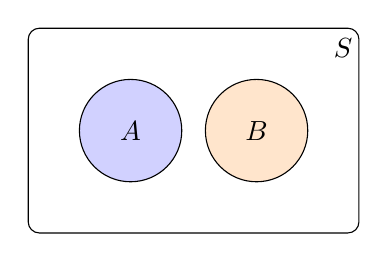
\begin{tikzpicture}[x=1cm,y=1cm]
                \draw[rounded corners] (0,0) rectangle (4.2,2.6);
                \node at (4.0,2.35) {$S$};
                \draw[fill=blue!18] (1.3,1.3) circle (0.65);
                \draw[fill=orange!20] (2.9,1.3) circle (0.65);
                \node at (1.3,1.3) {$A$};
                \node at (2.9,1.3) {$B$};
            \end{tikzpicture}
        \end{column}
        \begin{column}{0.48\textwidth}
            \textbf{Bağımsız (Independent)}
            \begin{itemize}
                \item \(P(A\cap B)=P(A)P(B)\)
                \item Kesişim boş olmak zorunda değildir
                \item Bilgi etkisi yoktur
            \end{itemize}
            \centering
            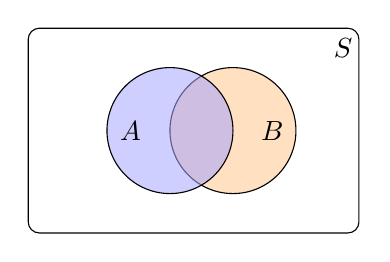
\begin{tikzpicture}[x=1cm,y=1cm]
                \draw[rounded corners] (0,0) rectangle (4.2,2.6);
                \node at (4.0,2.35) {$S$};
                \draw[fill=orange!45, fill opacity=0.55] (2.6,1.3) circle (0.8);
                \draw[fill=blue!35, fill opacity=0.55] (1.8,1.3) circle (0.8);
                \node at (1.3,1.3) {$A$};
                \node at (3.1,1.3) {$B$};
            \end{tikzpicture}
        \end{column}
    \end{columns}

    \vspace{0.15cm}
    \begin{block}{Neden çelişir?}
        Ayrıksa $P(A\cap B)=0$, ama bağımsızlık $P(A)P(B)>0$ gerektirir. $0 \neq P(A)P(B)$ $\Rightarrow$ çelişki.
    \end{block}
\end{frame}

\begin{frame}{Somut Örnek: Ayrıklık vs Bağımsızlık}
    \begin{columns}[T]
        \begin{column}{0.48\textwidth}
            \begin{block}{\faLink\ Ayrık Olaylar (Disjoint)}
                \textbf{\textit{``Bu olduysa diğeri OLAMAZ''}}
                \vspace{0.2cm}
                
                \textbf{Senaryo:} Bir arabanın durumu.
                \begin{itemize}
                    \item \(A\): Araba çalışıyor.
                    \item \(B\): Araba tamamen bozuk.
                \end{itemize}
                
                \textbf{Analiz:}
                \begin{itemize}
                    \item Araba aynı anda hem çalışıp hem bozuk olamaz.
                    \item Kesişim İMKANSIZDIR ($P(A\cap B)=0$).
                    \item Birinin bilinmesi diğerini \%100 etkiler (Bozuksa çalışmıyordur).
                \end{itemize}
            \end{block}
        \end{column}
        \begin{column}{0.48\textwidth}
            \begin{block}{\faUnlink\ Bağımsız Olaylar (Independent)}
                \textbf{\textit{``Bu olduysa diğeri FARK ETMEZ''}}
                \vspace{0.2cm}
                
                \textbf{Senaryo:} İki farklı arabanın durumu.
                \begin{itemize}
                    \item \(A\): İstanbul'daki araba çalışıyor.
                    \item \(B\): Ankara'daki araba bozuk.
                \end{itemize}
                
                \textbf{Analiz:}
                \begin{itemize}
                    \item İstanbul'daki durum Ankara'dakini etkilemez.
                    \item İkisi aynı anda olabilir ($P(A\cap B) \neq 0$).
                    \item Birini bilmek diğeri hakkında bilgi vermez.
                \end{itemize}
            \end{block}       
        \end{column}
    \end{columns}
\end{frame}

\begin{frame}[fragile]{Bağımsızlıkta Çarpım Kuralı}
    Genel çarpım:
    \[
    P(A\cap B)=P(A)P(B|A)
    \]
    Bağımsızlıkta:
    \[
    P(B|A)=P(B)\quad \Rightarrow\quad P(A\cap B)=P(A)P(B).
    \]

    \begin{block}{Hızlı Test}
        Verilerden \(P(A\cap B)\) ile \(P(A)P(B)\) eşitse bağımsızlık vardır.
    \end{block}
\end{frame}

\begin{frame}{Örnek 2.38: İtfaiye ve Ambulans}
    \small
    Küçük bir kasabada bir itfaiye aracı ve bir ambulans bulunmaktadır. Acil bir durumda araçların hazır olma olasılıkları birbirinden bağımsızdır:
    \begin{itemize}
        \item İtfaiye aracının hazır olma olasılığı: $P(I) = 0.98$
        \item Ambulansın hazır olma olasılığı: $P(A) = 0.92$
    \end{itemize}

    \only<1>{
        \footnotesize
        \begin{block}{Çözüm İskeleti}
            Hedef olay \(I \cap A\)'dır. Soruda bağımsızlık verildiği için doğrudan
            \(P(I \cap A)=P(I)P(A)\) kullanılır.
        \end{block}
    }

    \vspace{0.2cm}
    \textbf{Soru:} Bir kaza anında \textbf{her iki} aracın da hazır olma olasılığı nedir?

    \onslide<2->{
        \textbf{Çözüm:} Olaylar bağımsız olduğu için kesişim çarpıma eşittir:
        \[ P(I \cap A) = P(I) \cdot P(A) \]
        \[ P(I \cap A) = (0.98)(0.92) = 0.9016 \]
    }
\end{frame}

\subsection{Pekiştirme Soruları (Sıra Sizde)}

\begin{frame}{Soru 2: Yedek Güç Ünitesi (Bağımsızlık)}
    Bir veri merkezinde iki bağımsız yedek güç ünitesi (Jeneratör A ve Jeneratör B) bulunmaktadır.
    \begin{itemize}
        \item Jeneratör A'nın başarıyla çalışması: $P(A) = 0.90$
        \item Jeneratör B'nin başarıyla çalışması: $P(B) = 0.80$
    \end{itemize}

    \textbf{Soru:} Elektrik kesintisi olduğunda;
    \begin{enumerate}
        \item[(a)] Her iki jeneratörün de aynı anda çalışması ($A \cap B$) olasılığı nedir?
        \item[(b)] Sistemin tamamen enerjisiz kalması (ikisinin de çalışmaması) olasılığı nedir?
        \item[(c)] En az bir jeneratörün çalışması ($A \cup B$) olasılığı nedir?
    \end{enumerate}
\end{frame}

\begin{frame}{Soru 2: Çözüm}
    \vspace{5cm}
\end{frame}

\begin{frame}[allowframebreaks]{Soru 2: Detaylı Çözüm}
    \small
    {\color{red}
    \textbf{Verilenler:} \(P(A)=0.90\), \(P(B)=0.80\), olaylar bağımsız.

    \textbf{(a) Her iki jeneratörün de çalışması}
    \[
    P(A\cap B)=P(A)P(B)=(0.90)(0.80)=\mathbf{0.72}
    \]

    \textbf{(b) Sistemin tamamen enerjisiz kalması}
    \[
    P(A')=0.10,\qquad P(B')=0.20
    \]
    Bağımsızlık tamamlayıcılara da taşınır:
    \[
    P(A'\cap B')=P(A')P(B')=(0.10)(0.20)=\mathbf{0.02}
    \]

    \textbf{(c) En az bir jeneratörün çalışması}
    \[
    P(A\cup B)=1-P(A'\cap B')=1-0.02=\mathbf{0.98}
    \]

    \textbf{Sonuç:} Sistem kesinti anında \(\%98\) olasılıkla en az bir kaynakla enerji sağlar.
    }
\end{frame}



\begin{frame}{Bağımsızlıkta Kontrol Listesi}
    \begin{enumerate}
        \item \textbf{Otomatik varsaymayın:} Soruda ``bağımsız'' açıkça belirtilmedikçe bağımsızlık varsayımı yapmayın.
        \item \textbf{Ayrıklık $\neq$ Bağımsızlık:} Ayrık olaylar ($A\cap B=\emptyset$) pozitif olasılıklıysa bağımsız olamaz.
        \item \textbf{Sayısal test yapın:} Elinizde yeterli veri varsa \(P(A\cap B)\stackrel{?}{=}P(A)P(B)\) eşitliğini doğrudan kontrol edin.
    \end{enumerate}
\end{frame}

\begin{frame}{Sayısal Test Nasıl Yapılır? (Örnekler)}
    \begin{columns}[T]
        \begin{column}{0.48\textwidth}
            \begin{exampleblock}{Örnek 1: Bağımsızlık Var}
                \small
                \textbf{Veri:} $P(A)=0.4$, $P(B)=0.5$, $P(A \cap B)=0.2$.
                
                \textbf{Test:}
                \[ P(A) \cdot P(B) \stackrel{?}{=} P(A \cap B) \]
                \[ 0.4 \cdot 0.5 = 0.2 \]
                \[ 0.2 = 0.2 \quad \text{\faCheck} \]
                
                \textbf{Sonuç:} Eşitlik sağlandığı için olaylar \textbf{bağımsızdır}.
            \end{exampleblock}
        \end{column}
        \begin{column}{0.48\textwidth}
            \begin{alertblock}{Örnek 2: Bağımlılık Var}
                \small
                \textbf{Veri:} $P(A)=0.4$, $P(B)=0.5$, $P(A \cap B)=0.1$.
                
                \textbf{Test:}
                \[ P(A) \cdot P(B) \stackrel{?}{=} P(A \cap B) \]
                \[ 0.4 \cdot 0.5 = 0.2 \]
                \[ 0.2 \neq 0.1 \quad \text{\faTimes} \]
                
                \textbf{Sonuç:} Eşitlik bozulduğu için olaylar \textbf{bağımlıdır}.
            \end{alertblock}
        \end{column}
    \end{columns}
\end{frame}

\section{Tam Bağımsızlık (Total Independence)}
\subsection{İkili Bağımsızlık ve Tam Bağımsızlık}

\begin{frame}{Neden İkili Bağımsızlık Yetmez?}
    Üç olay \(A,B,C\) için sadece
    \[
    P(A\cap B)=P(A)P(B),\;
    P(A\cap C)=P(A)P(C),\;
    P(B\cap C)=P(B)P(C)
    \]
    olması yeterli değildir.

    \begin{block}{Tam Bağımsızlık}
        Her alt kümede çarpım kuralı sağlanmalıdır.
    \end{block}
\end{frame}

\begin{frame}{Tanım: Karşılıklı Bağımsızlık (Definition 2.12)}
    Üç olay için gereken tüm koşullar:
    \begin{enumerate}
        \item \(P(A\cap B)=P(A)P(B)\)
        \item \(P(A\cap C)=P(A)P(C)\)
        \item \(P(B\cap C)=P(B)P(C)\)
        \item \(P(A\cap B\cap C)=P(A)P(B)P(C)\)
    \end{enumerate}

    \begin{block}{Genelleme}
        $n$ olay için tam bağımsızlık toplam $2^n - n - 1$ koşul gerektirir.\\
        \textbf{Örnekler:} 3~olay $\rightarrow$ 4~koşul,\quad 4~olay $\rightarrow$ 11~koşul,\quad 5~olay $\rightarrow$ 26~koşul.\\
        Sadece ikili eşitlikler (1--3) yetmez; üçlü (4) ayrıca sağlanmalıdır.
    \end{block}
\end{frame}

\begin{frame}[fragile]{Karşı Örnek: İkili Bağımsızlık Var, Tamı Yok}
    \footnotesize
    \begin{columns}[T,onlytextwidth]
        \begin{column}{0.49\textwidth}
            \textbf{Deney Tanımı:} İki adil para atışı, \(S=\{YY,YT,TY,TT\}\).\\
            \textit{Not:} \(Y\)=Yazı, \(T\)=Tura.
            \[
            A=\{\text{ilk atış }Y\},\quad
            B=\{\text{ikinci atış }Y\},\quad
            C=\{\text{iki atış aynı}\}
            \]

            \textbf{Olasılıklar:}
            \begin{itemize}\itemsep2pt
                \item \(P(A)=P(B)=P(C)=\tfrac{1}{2}\)
                \item \(P(A\cap B)=P(A\cap C)=P(B\cap C)=\tfrac{1}{4}\)
            \end{itemize}
            Tüm ikili kombinasyonlar bağımsızdır.
        \end{column}
        \begin{column}{0.49\textwidth}
            \begin{alertblock}{Üçlü Kesişim Analizi}
                \textbf{Neden \(P(A \cap B \cap C)=\tfrac{1}{4}\)?}
                \begin{itemize}\itemsep2pt
                    \item \(A \cap B = \{YY\}\)
                    \item \(YY\) gerçekleştiğinde \(C\) otomatik sağlanır.
                    \item \((A \cap B) \cap C = \{YY\}\)
                \end{itemize}
                \[
                P(A \cap B \cap C)=\tfrac{1}{4},\qquad
                P(A)P(B)P(C)=\tfrac{1}{8}
                \]
                \[
                \tfrac{1}{4} \neq \tfrac{1}{8}\Rightarrow \text{tam bağımsız değil.}
                \]
            \end{alertblock}
        \end{column}
    \end{columns}

    \[
    \boxed{\text{İkili bağımsızlık var, tam bağımsızlık yok.}}
    \]
\end{frame}

\begin{frame}{Örnek 2.39: Seri ve Paralel Devreler}
    \begin{columns}[T]
        \begin{column}{0.55\textwidth}
            \textbf{Soru:}
            Şekildeki gibi bir devrede bileşenlerin çalışma olasılıkları $P(C_1)=0.9$, $P(C_2)=0.9$, $P(C_3)=0.8$'dir ve birbirlerinden bağımsızdır. Devrenin (sistemin) çalışma olasılığı nedir?

            \vspace{0.2cm}
            \centering
            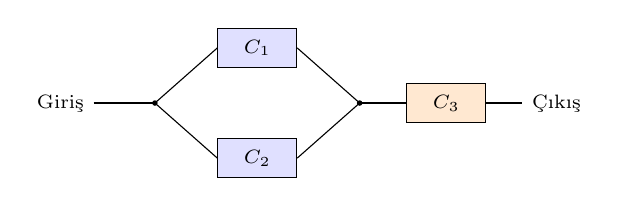
\begin{tikzpicture}[x=1cm,y=1cm,>=stealth,every node/.style={font=\scriptsize}]
                % Dalların ayrıştığı ve birleştiği düğümler
                \coordinate (split) at (1.2,0.5);
                \coordinate (merge) at (3.8,0.5);

                % Bileşenler (C1 ve C2 merkez etrafında simetrik)
                \node[draw, fill=blue!12, minimum width=1cm, minimum height=0.5cm] (c1) at (2.5,1.2) {$C_1$};
                \node[draw, fill=blue!12, minimum width=1cm, minimum height=0.5cm] (c2) at (2.5,-0.2) {$C_2$};
                \node[draw, fill=orange!18, minimum width=1cm, minimum height=0.5cm] (c3) at (4.9,0.5) {$C_3$};

                % Giriş/çıkış etiketleri
                \node (in) at (0,0.5) {Giriş};
                \node (out) at (6.3,0.5) {Çıkış};

                % Bağlantılar (anchor kullanarak kutulara tam temas)
                \draw (in.east) -- (split);
                \draw (split) -- (c1.west);
                \draw (split) -- (c2.west);
                \draw (c1.east) -- (merge);
                \draw (c2.east) -- (merge);
                \draw (merge) -- (c3.west);
                \draw (c3.east) -- (out.west);

                % Düğüm noktalarını görünür yap
                \fill (split) circle (1pt);
                \fill (merge) circle (1pt);
            \end{tikzpicture}
        \end{column}
        \begin{column}{0.44\textwidth}
            \onslide<2->{
                \textbf{Çözüm:}
                \small
                \begin{itemize}
                    \item \textbf{Paralel Kısım ($A$):} $C_1 \cup C_2$.
                    $P(A) = 1 - P(C_1' \cap C_2')$
                    $P(A) = 1 - (0.1)(0.1) = 0.99$.

                    \item \textbf{Tüm Sistem:} $A \cap C_3$ (Seri).
                    $A$, sadece $(C_1,C_2)$ olaylarının bir fonksiyonudur; $C_3$ ise bu ikisinden bağımsız verildiği için $A$ ile $C_3$ bağımsızdır.
                    $P(\text{Sistem}) = P(A) \cdot P(C_3)$
                    $P(\text{Sistem}) = 0.99 \cdot 0.8 = 0.792$.
                \end{itemize}
            }
        \end{column}
    \end{columns}
\end{frame}

\subsection{Pekiştirme Soruları (Sıra Sizde)}

\begin{frame}{Soru 3: Gelişmiş Sistem Güvenilirliği}
    \small
    Beş bileşenli ($K_1 - K_5$) bir sistemin yapısı şöyledir:
    \begin{itemize}
        \item \textbf{Ana Yapı:} Üç ana kol ($Kol_1, Kol_2, Kol_3$) birbirine \textbf{paraleldir}.
        \item \textbf{Kol 1:} $K_1$ bileşeni, ($K_2$ ve $K_3$'ün paralel olduğu) bir bloğa \textbf{seri} bağlıdır.
        \item \textbf{Kol 2:} Sadece $K_4$ bileşeni vardır.
        \item \textbf{Kol 3:} Sadece $K_5$ bileşeni vardır.
    \end{itemize}

    \textbf{Bozulma Olasılıkları (Bağımsız):}
    $P(K_1')=0.05, P(K_2')=0.10, P(K_3')=0.10, P(K_4')=0.20, P(K_5')=0.20$.

    \vspace{0.2cm}
    \begin{columns}[T]
        \begin{column}{0.45\textwidth}
            \textbf{Sorular:}
            \begin{enumerate}
                \item[(a)] Sistemin \textbf{TAMAMEN bozulma} olasılığı nedir?
                \item[(b)] Sistemin \textbf{çalışma} olasılığı nedir?
            \end{enumerate}
        \end{column}
        \begin{column}{0.50\textwidth}
            \centering
            % TikZ Devre Şeması
            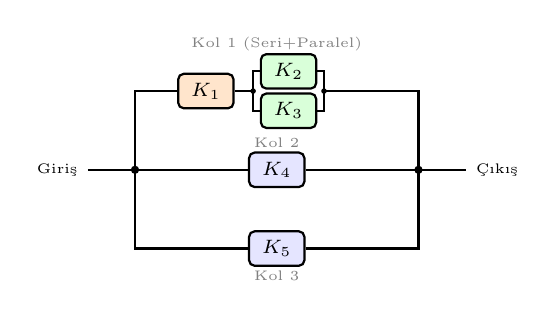
\begin{tikzpicture}[x=0.6cm,y=0.5cm,>=stealth, line width=0.8pt]
                \tikzstyle{block} = [draw, fill=blue!10, rectangle, minimum height=1.2em, minimum width=2em, rounded corners=2pt, font=\scriptsize]
                
                % Giriş Düğümü
                \coordinate (input) at (0,0);
                \coordinate (split) at (1,0);
                \coordinate (merge) at (7,0);
                \coordinate (output) at (8,0);

                % Ana Hatlar
                \draw (input) -- (split);
                \draw (merge) -- (output) node[right] {\tiny Çıkış};
                \draw (input) node[left] {\tiny Giriş};

                % Kol 1 (Üst - Karmaşık)
                \draw (split) -- (1, 2) -- (2, 2);
                \node[block, fill=orange!20] (k1) at (2.5, 2) {$K_1$};
                \draw (k1.east) -- (3.5, 2);
                
                % Kol 1 - Paralel Alt Kısım
                % Önce node'ları oluştur
                \node[block, fill=green!15] (k2) at (4.25, 2.5) {$K_2$};
                \node[block, fill=green!15] (k3) at (4.25, 1.5) {$K_3$};
                
                % Sonra çizgileri çiz (böylece çizgiler node'ların üstünde görünür)
                \draw (3.5, 2) -- (3.5, 2.5) -- (k2.west);
                \draw (k2.east) -- (5, 2.5) -- (5, 2);

                \draw (3.5, 2) -- (3.5, 1.5) -- (k3.west);
                \draw (k3.east) -- (5, 1.5) -- (5, 2);
                
                \draw (5, 2) -- (7, 2) -- (merge);

                % Kol 2 (Orta - Basit)
                \node[block] (k4) at (4, 0) {$K_4$};
                \draw (split) -- (k4.west);
                \draw (k4.east) -- (merge);

                % Kol 3 (Alt - Basit)
                \draw (split) -- (1, -2) -- (3.5, -2);
                \node[block] (k5) at (4, -2) {$K_5$};
                \draw (k5.east) -- (7, -2) -- (merge);

                % Etiketler
                \node[font=\tiny, gray] at (4, 3.2) {Kol 1 (Seri+Paralel)};
                \node[font=\tiny, gray] at (4, 0.7) {Kol 2};
                \node[font=\tiny, gray] at (4, -2.7) {Kol 3};

                % Node noktaları
                \fill[black] (split) circle (1.5pt);
                \fill[black] (merge) circle (1.5pt);
                \fill[black] (3.5, 2) circle (1pt);
                \fill[black] (5, 2) circle (1pt);
            \end{tikzpicture}
        \end{column}
    \end{columns}
\end{frame}

\begin{frame}[allowframebreaks]{Soru 3: Detaylı Çözüm}
    \small
    {\color{red}
    \textbf{Strateji:} Sistem paralel ana kollardan oluştuğu için, sistemin \textbf{bozulması} demek \textbf{TÜM kolların} aynı anda bozulması demektir.
    \[ P(S') = P(Kol_1') \times P(Kol_2') \times P(Kol_3') \]

    \textbf{1. Adım: Kol 1'in Analizi}
    \begin{itemize}
        \item $K_2$ ve $K_3$ paralel: $P(\text{alt bozuk}) = P(K_2')P(K_3') = (0.10)(0.10) = 0.01$.
        \item Bu alt grup ($0.01$) ile $K_1$ ($0.05$) \textbf{seri} bağlıdır.
        \item Seri yapıda \textbf{çalışma} olasılıkları çarpılır:
        \[ R_{alt} = 1 - 0.01 = 0.99, \quad R_{K1} = 1 - 0.05 = 0.95 \]
        \[ R_{Kol1} = 0.95 \times 0.99 = 0.9405 \]
        \item Kol 1 Bozulma: $P(Kol_1') = 1 - 0.9405 = \mathbf{0.0595}$.
    \end{itemize}

    \textbf{2. Adım: Diğer Kollar}
    \begin{itemize}
        \item $P(Kol_2') = P(K_4') = \mathbf{0.20}$
        \item $P(Kol_3') = P(K_5') = \mathbf{0.20}$
    \end{itemize}

    \textbf{3. Adım: Sistem Sonucu}
    \[
    \textbf{(a) } P(S') = (0.0595) \times (0.20) \times (0.20) = 0.0595 \times 0.04 = \mathbf{0.00238}
    \]
    \[
    \textbf{(b) } P(S) = 1 - P(S') = 1 - 0.00238 = \mathbf{0.99762}
    \]
    
    Yani sistem yaklaşık \textbf{\%99.76} güvenilirliktedir.
    }
\end{frame}

\section{Toplam Olasılık Teoremi}
\subsection{Parçalama (Partition) ve Teorem}

\begin{frame}{Parçalanış (Partition) Nedir?}
    \begin{columns}[T]
        \begin{column}{0.58\textwidth}
            \begin{block}{Tanım}
                \(S\) örnek uzayı, \(B_1,\dots,B_k\) olaylarıyla parçalanıyorsa:
                \begin{enumerate}
                    \item \(i\neq j\) için \(B_i\cap B_j=\emptyset\),
                    \item \(\bigcup_{i=1}^{k} B_i=S\),
                    \item her \(i\) için \(P(B_i)>0\).
                \end{enumerate}
            \end{block}
            \textbf{Amaç:} Karmaşık olayı örtüşmeyen alt senaryolara ayırmak.
        \end{column}
        \begin{column}{0.40\textwidth}
            \centering
            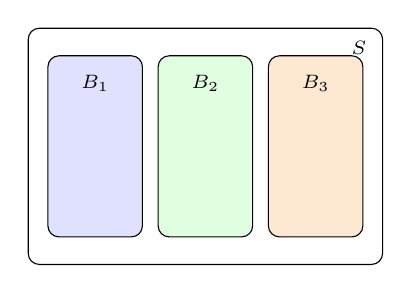
\begin{tikzpicture}[x=1cm,y=1cm,every node/.style={font=\scriptsize}]
                \draw[rounded corners] (0,0) rectangle (4.5,3.0);
                \node at (4.2,2.75) {$S$};
                \draw[fill=blue!12,rounded corners] (0.25,0.35) rectangle (1.45,2.65);
                \draw[fill=green!12,rounded corners] (1.65,0.35) rectangle (2.85,2.65);
                \draw[fill=orange!18,rounded corners] (3.05,0.35) rectangle (4.25,2.65);
                \node at (0.85,2.3) {$B_1$};
                \node at (2.25,2.3) {$B_2$};
                \node at (3.65,2.3) {$B_3$};
            \end{tikzpicture}
        \end{column}
    \end{columns}
\end{frame}

\begin{frame}{Olayların Parçalanması}
    Herhangi bir $A$ olayı, partition elemanlarıyla kesişimlerin birleşimi olarak yazılabilir:
    \[
    A = (B_1 \cap A) \cup (B_2 \cap A) \cup \cdots \cup (B_k \cap A)
    \]

    Bu kesişimler ($B_i \cap A$) birbirleriyle \textbf{ayrık} oldukları için, $A$'nın toplam olasılığı bu parçaların olasılıklarının toplamıdır:
    \[
    P(A) = P(B_1 \cap A) + P(B_2 \cap A) + \cdots + P(B_k \cap A)
    \]

    \begin{block}{Sonraki adım}
        Her $P(B_i \cap A)$ terimini çarpım kuralıyla açarsak Toplam Olasılık Teoremine ulaşırız.
    \end{block}
\end{frame}

\begin{frame}[fragile]{Toplam Olasılık Teoremi (Theorem 2.13)}
    \begin{block}{Teorem}
        \(B_1,\dots,B_k\) bir partition ise:
        \[
        P(A)=\sum_{i=1}^{k}P(B_i\cap A)=\sum_{i=1}^{k}P(B_i)P(A|B_i).
        \]
    \end{block}

    \begin{itemize}
        \item Her terim: ``dal olasılığı'' (\(P(B_i)\times P(A|B_i)\)).
        \item Toplam: \(A\)'ya giden tüm yolların toplamı.
    \end{itemize}
\end{frame}


\begin{frame}{Örnek 2.41: Montaj Fabrikası}
    \small
    \begin{columns}[T]
        \begin{column}{0.55\textwidth}
            \textbf{Soru:}
            Bir fabrikada üç makine ($B_1, B_2, B_3$) üretim yapmaktadır.
            \begin{itemize}
                \item Üretim payları: $B_1: \%30, \, B_2: \%45, \, B_3: \%25$.
                \item Hatalı ürün ($A$) oranları: $P(A|B_1)=0.02,\; P(A|B_2)=0.03,\; P(A|B_3)=0.02$.
            \end{itemize}
            Rastgele seçilen bir ürünün \textbf{hatalı} olma olasılığı nedir?
            
            \onslide<2->{
                \vspace{0.3cm}
                \footnotesize
                \textbf{Notasyon Analizi:}
                \begin{itemize}
                    \item $B_1, B_2, B_3$: Ürünün geldiği makine olayları.
                    \item $A$: Seçilen ürünün \textbf{hatalı} olması olayı.
                    \item $P(B_1)=0.30$: 1. Makinenin üretim payı.
                    \item $P(A|B_1)=0.02$: Sadece 1 numaralı makinenin üretim yaptığı ön koşulundaki hata oranı.
                \end{itemize}
            }
        \end{column}
        \begin{column}{0.44\textwidth}
            \only<1-2>{
                \footnotesize
                \begin{block}{Çözüm İskeleti}
                    Partition kontrolü $\rightarrow$
                    $P(A)=\sum_i P(B_i)P(A|B_i)$ uygula $\rightarrow$
                    terim katkılarını kıyasla.
                \end{block}
            }

            \onslide<3->{
                \textbf{Çözüm:}
                Toplam Olasılık Teoremini uygulayalım:
                \[ P(A) = \sum P(B_i)P(A|B_i) \]

                \footnotesize
                \begin{align*}
                P(A)&=0.30(0.02)+0.45(0.03)+0.25(0.02)\\
                    &=0.0245
                \end{align*}
                \[
                \mathbf{P(A)=0.0245=\%2.45}
                \]
            }
        \end{column}
    \end{columns}
\end{frame}




\begin{frame}{Toplam Olasılık: Ağaç Diyagramı Okuma}
    \begin{columns}[T]
        \begin{column}{0.48\textwidth}
            \begin{block}{Yol mantığı}
                $A$ olayı farklı kaynaklardan ($B_1,B_2,B_3$) gelebilir:
                \[
                P(A)=\sum_i P(B_i)P(A|B_i).
                \]
                Her terim, ağaçta bir dalın \textbf{çarpım} olasılığıdır.
            \end{block}
            \begin{itemize}
                \item Önce ``hangi kaynak?'' dalı seçilir.
                \item Sonra ``o kaynakta $A$ oldu mu?'' dalı seçilir.
                \item $A$'ya giden tüm yollar toplanır.
            \end{itemize}
        \end{column}
        \begin{column}{0.48\textwidth}
            \centering
            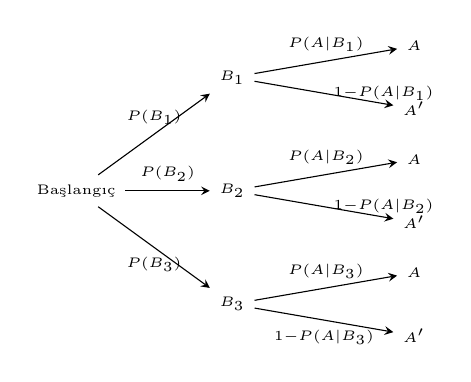
\begin{tikzpicture}[x=1.1cm,y=0.8cm,>=stealth, every node/.style={font=\tiny}]
                \node (r) at (0,0) {Başlangıç};
                \node (b1) at (1.8,1.8) {$B_1$};
                \node (b2) at (1.8,0.0) {$B_2$};
                \node (b3) at (1.8,-1.8) {$B_3$};

                \draw[->] (r)--(b1) node[midway,above] {$P(B_1)$};
                \draw[->] (r)--(b2) node[midway,above] {$P(B_2)$};
                \draw[->] (r)--(b3) node[midway,below] {$P(B_3)$};

                \node (a1) at (3.9,2.3) {$A$};
                \node (c1) at (3.9,1.3) {$A'$};
                \node (a2) at (3.9,0.5) {$A$};
                \node (c2) at (3.9,-0.5) {$A'$};
                \node (a3) at (3.9,-1.3) {$A$};
                \node (c3) at (3.9,-2.3) {$A'$};

                \draw[->] (b1)--(a1) node[midway,above] {$P(A|B_1)$};
                \draw[->] (b1)--(c1) node[midway,right] {$1{-}P(A|B_1)$};
                \draw[->] (b2)--(a2) node[midway,above] {$P(A|B_2)$};
                \draw[->] (b2)--(c2) node[midway,right] {$1{-}P(A|B_2)$};
                \draw[->] (b3)--(a3) node[midway,above] {$P(A|B_3)$};
                \draw[->] (b3)--(c3) node[midway,below] {$1{-}P(A|B_3)$};
            \end{tikzpicture}
        \end{column}
    \end{columns}
\end{frame}

% ------------------------------------------------------------
% SORU: Ağaç diyagramı (Banttan alınma olayı A)
% ------------------------------------------------------------
\begin{frame}{Örnek: Ağaç Diyagramı (Kalite Kontrol)}
\small
\begin{columns}[T]
\begin{column}{0.48\textwidth}
Bir üretim bandından geçen mamüller:
\[
B_1:\ \text{çok kusurlu},\quad
B_2:\ \text{az kusurlu},\quad
B_3:\ \text{kusursuz}.
\]

Önsel olasılıklar:
\[
P(B_1)=0.05,\quad P(B_2)=0.10,\quad P(B_3)=0.85.
\]

Çalışanlar kusurlu gördüklerini banttan alıyor:
\[
A:\ \text{``banttan alınma''}.
\]

Koşullu olasılıklar (diyagrama göre):
\[
P(A\mid B_1)=0.98,\quad P(A\mid B_2)=0.40,\quad P(A\mid B_3)=0.01.
\]
\end{column}

\begin{column}{0.48\textwidth}
\textbf{Soru:} Banttan alınan bir mamülün
\(\,P(B_1\mid A),\,P(B_2\mid A),\,P(B_3\mid A)\,\)
olasılıklarını bulunuz.

\centering
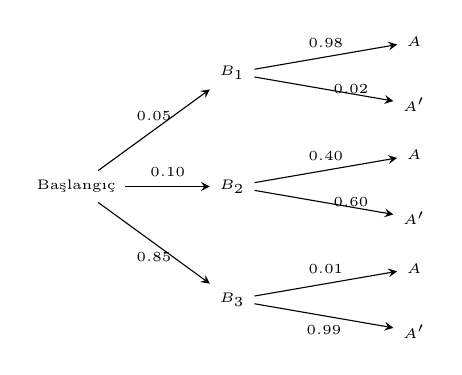
\begin{tikzpicture}[x=1.1cm,y=0.8cm,>=stealth, every node/.style={font=\tiny}]
    \node (r) at (0,0) {Başlangıç};
    \node (b1) at (1.8,1.8) {$B_1$};
    \node (b2) at (1.8,0.0) {$B_2$};
    \node (b3) at (1.8,-1.8) {$B_3$};

    \draw[->] (r)--(b1) node[midway,above] {$0.05$};
    \draw[->] (r)--(b2) node[midway,above] {$0.10$};
    \draw[->] (r)--(b3) node[midway,below] {$0.85$};

    \node (a1) at (3.9,2.3) {$A$};
    \node (c1) at (3.9,1.3) {$A'$};
    \node (a2) at (3.9,0.5) {$A$};
    \node (c2) at (3.9,-0.5) {$A'$};
    \node (a3) at (3.9,-1.3) {$A$};
    \node (c3) at (3.9,-2.3) {$A'$};

    \draw[->] (b1)--(a1) node[midway,above] {$0.98$};
    \draw[->] (b1)--(c1) node[midway,right] {$0.02$};
    \draw[->] (b2)--(a2) node[midway,above] {$0.40$};
    \draw[->] (b2)--(c2) node[midway,right] {$0.60$};
    \draw[->] (b3)--(a3) node[midway,above] {$0.01$};
    \draw[->] (b3)--(c3) node[midway,below] {$0.99$};
\end{tikzpicture}
\end{column}
\end{columns}
\end{frame}


% ------------------------------------------------------------
% ÇÖZÜM: Toplam olasılık + Bayes

\begin{frame}{Çözüm: Ağaç Diyagramı ile Bayes (1/2)}
\small

\begin{block}{1) Önce $P(A)$ (Toplam Olasılık)}
\begin{equation}
\label{eq:PA_tree}
P(A)=\sum_{i=1}^3 P(A\mid B_i)\,P(B_i)
=0.98\cdot 0.05 + 0.40\cdot 0.10 + 0.01\cdot 0.85
=0.0975.
\end{equation}
\end{block}

\begin{alertblock}{2) Bayes formülü}
\begin{equation}
\label{eq:posterior_tree}
P(B_i\mid A)=\frac{P(A\mid B_i)\,P(B_i)}{P(A)} \qquad (i=1,2,3).
\end{equation}
\end{alertblock}

\begin{block}{3) İlk posterior hesap}
\[
P(B_1\mid A)=\frac{0.98\cdot 0.05}{0.0975}
=\frac{0.049}{0.0975}
=\frac{98}{195}\approx 0.503
\]
\end{block}

\end{frame}

\begin{frame}{Çözüm: Ağaç Diyagramı ile Bayes (2/2)}
\small

\begin{columns}[T]
\begin{column}{0.48\textwidth}
\begin{block}{$B_2$ için}
\[
P(B_2\mid A)=\frac{0.40\cdot 0.10}{0.0975}
=\frac{0.04}{0.0975}
=\frac{16}{39}\approx 0.410
\]
\end{block}
\end{column}

\begin{column}{0.48\textwidth}
\begin{block}{$B_3$ için}
\[
P(B_3\mid A)=\frac{0.01\cdot 0.85}{0.0975}
=\frac{0.0085}{0.0975}
=\frac{17}{195}\approx 0.087
\]
\end{block}
\end{column}
\end{columns}

\begin{alertblock}{Yorum}
Banttan alınan mamulün en olası durumu
\(\approx 50.3\%\) ile \textbf{çok kusurlu} çıkmasıdır.
\end{alertblock}

\end{frame}





\begin{frame}{Neden Toplam Olasılık? (Ayrıklık Prensibi)}
    \begin{alertblock}{Kritik Ayrım: Ayrıklık (Disjointness)}
        Bu soruda formülün \textbf{toplama} işlemi üzerine kurulmasının temel nedeni fiziksel gerçekliktir:
        \textbf{Bir ürün aynı anda farklı makinelerden beraber üretilmiş olamaz.}
    \end{alertblock}

    \vspace{0.5cm}
    \begin{columns}[T]
        \begin{column}{0.48\textwidth}
            \centering
            \textbf{\textcolor{red}{\faTimes\ Bu Değil (Ortak Üretim)}}
            \par\noindent\rule{0.8\textwidth}{0.4pt}
            \vspace{0.2cm}
            \scriptsize
            Yanlış Düşünce: ``Ürün hem Makine 1 hem Makine 2 tarafından yapıldı.''
            \[ B_1 \cap B_2 \neq \emptyset \]
            \textit{Bu mantıkta olsaydı, karmaşık kesişim formülleri kullanılırdı.}
        \end{column}
        \begin{column}{0.48\textwidth}
            \centering
            \textbf{\textcolor{green!60!black}{\faCheck\ Budur (Ayrık Üretim)}}
            \par\noindent\rule{0.8\textwidth}{0.4pt}
            \vspace{0.2cm}
            \scriptsize
            Doğru Gerçeği: ``Ürün YA Makine 1'den YA Makine 2'den gelir.''
            \[ B_1 \cap B_2 = \emptyset \]
            
            Olaylar birbirini dışladığı (ayrık olduğu) için olasılıklar \textbf{toplanır}:
            \[ P(A) = \sum P(A \cap B_i) \]
        \end{column}
    \end{columns}
\end{frame}

\subsection{Pekiştirme Soruları (Sıra Sizde)}

\begin{frame}{Soru 1: Otel Zinciri (Toplam Olasılık)}
    Büyük bir sanayi firması, misafirlerini konaklatmak için üç yerel otel kullanmaktadır. Geçmiş verilere göre:
    \begin{itemize}
        \item Ramada Inn'e gönderilme olasılığı: \%20
        \item Sheraton'a gönderilme olasılığı: \%50
        \item Lakeview Motor Lodge'a gönderilme olasılığı: \%30
    \end{itemize}

    Otellerdeki tesisat arızası (faulty plumbing) oranları ise şöyledir:
    \begin{itemize}
        \item Ramada Inn: \%5
        \item Sheraton: \%4
        \item Lakeview Motor Lodge: \%8
    \end{itemize}

    \textbf{Soru:} Rastgele seçilen bir müşterinin, tesisatı arızalı bir odaya denk gelme olasılığı nedir?
\end{frame}

\begin{frame}{Soru 1: Çözüm}
    \vspace{5cm}
\end{frame}

\begin{frame}[allowframebreaks]{Soru 1: Detaylı Çözüm}
    \footnotesize
    {\color{red}
    \textbf{Adım 1 -- Olayları tanımla:}
    $A$: tesisat arızası, $R$: Ramada Inn, $S$: Sheraton, $L$: Lakeview.

    \textbf{Adım 2 -- Partition kontrolü:}
    $\{R,S,L\}$ ayrık ve $P(R)+P(S)+P(L)=0.20+0.50+0.30=1$ $\checkmark$

    \textbf{Adım 3 -- Toplam Olasılık Teoremini uygula:}
    \[
    P(A)=P(R)P(A|R)+P(S)P(A|S)+P(L)P(A|L)
    \]
    \[
    P(A)=0.20(0.05)+0.50(0.04)+0.30(0.08)
    \]
    \[
    P(A)=0.010+0.020+0.024=0.054
    \]
    \[
    \boxed{P(A)=0.054=\%5.4}
    \]
    \textbf{Adım 4 -- Yorumla:} Sonuç, her otelin arıza oranının kullanım payıyla ağırlıklandırılmış ortalamasıdır. Katkılar sırasıyla Ramada: $0.010$, Sheraton: $0.020$, Lakeview: $0.024$ olduğundan \textbf{en büyük katkı Lakeview'den} gelir.
    }
\end{frame}

\begin{frame}{Toplam Olasılıkta Sık Hata}
    \begin{enumerate}
        \item \textbf{Koşullu olasılıkları doğrudan toplamak.}
        \begin{itemize}
            \item \textcolor{red}{Yanlış:} $P(A)=P(A|B_1)+P(A|B_2)+P(A|B_3)$
            \item \textcolor{green!60!black}{Doğru:} $P(A)=\sum P(B_i)P(A|B_i)$
        \end{itemize}
        \item \textbf{Ağırlık çarpanlarını unutmak.}
        \begin{itemize}
            \item Her $P(A|B_i)$, ilgili $P(B_i)$ ile çarpılmalıdır.
        \end{itemize}
        \item \textbf{Partition olmayan kümelerle toplam yapmak.}
        \begin{itemize}
            \item $B_i$'ler örnek uzayı tam ve ayrık kapsamalıdır ($\sum P(B_i)=1$).
        \end{itemize}
    \end{enumerate}
\end{frame}

\section{Bayes Teoremi (Bayes' Rule)}
\subsection{Teorem ve Uygulama}

\begin{frame}[fragile]{Bayes Teoremi (Theorem 2.14)}
    \begin{block}{Formül}
        \(B_1,\dots,B_k\) bir partition ve \(P(A)>0\) ise:
        \[
        P(B_r|A)
        =
        \frac{P(B_r)P(A|B_r)}
        {\underbrace{\sum_{i=1}^{k}P(B_i)P(A|B_i)}_{\text{Toplam Olasılık } P(A)}}.
        \]
    \end{block}

    \begin{itemize}
        \item \textbf{Prior (Önsel):} \(P(B_r)\) -- Kanıt görmeden önceki inancımız.
        \item \textbf{Likelihood (Olabilirlik):} \(P(A|B_r)\) -- Bu kaynak doğruysa, gözlemi ne kadar iyi açıklar?
        \item \textbf{Posterior (Sonsal):} \(P(B_r|A)\) -- Kanıtı gördükten sonra güncellenen inancımız.
    \end{itemize}

    \vspace{0.15cm}
    \footnotesize
    \textit{Payda, bir önceki bölümde öğrendiğiniz Toplam Olasılık formülüdür.}
\end{frame}

\begin{frame}{Bayes'i Ezbersiz Okuma}
    \begin{block}{Kesişim / Toplam Mantığı}
        \[
        P(B_r|A)=\frac{P(B_r\cap A)}{P(A)}
        \]
        Yani ``ilgili yol'' / ``A'ya giden tüm yollar''.
    \end{block}

    \begin{itemize}
        \item Pay: hedef kaynaktan gelip gözlemi üretme.
        \item Payda: gözlemi üreten tüm kaynakların toplamı.
    \end{itemize}
\end{frame}

\begin{frame}{Sayım Tablosu ile Bayes: Kızamık--Lekeli}
    \small
    \begin{columns}[T]
        \begin{column}{0.58\textwidth}
            \centering
            \begin{tabular}{lcc|c}
                \toprule
                 & $L$ (Lekeli) & $L'$ & Toplam \\
                \midrule
                $K$ (Kızamık)   & $18$ & $2$  & $20$ \\
                $K'$            & $12$ & $68$ & $80$ \\
                \midrule
                Toplam          & $30$ & $70$ & $100$ \\
                \bottomrule
            \end{tabular}

            \vspace{0.2cm}
            \footnotesize
            Tablodaki sayılar bir örneklemden geliyor: Bayes'i ``sayarak'' kuracağız.
        \end{column}

        \begin{column}{0.40\textwidth}
            \begin{block}{Hedef}
                $P(K\mid L)$
            \end{block}

            \begin{alertblock}{Direkt oran (en sezgisel yol)}
                \[
                P(K\mid L)=\frac{\#(K\cap L)}{\#(L)}=\frac{18}{30}=0.6
                \]
            \end{alertblock}

            \begin{block}{Aynı sonucu Bayes ile yaz}
                \[
                P(K\mid L)=\frac{P(L\mid K)P(K)}{P(L)}
                =\frac{\tfrac{18}{20}\cdot\tfrac{20}{100}}{\tfrac{30}{100}}
                =\frac{0.9\times 0.2}{0.3}=0.6\;\checkmark
                \]
            \end{block}
        \end{column}
    \end{columns}
\end{frame}

\begin{frame}{Örnek 2.42: Hangi Makine? (Bayes Uygulaması)}
    \small
    \textbf{Soru:} Toplam Olasılık bölümündeki fabrika örneğinden (Örnek~2.41) devam ediyoruz. Rastgele seçilen bir ürünün \textbf{hatalı ($A$)} olduğu tespit edilmiştir. Bu ürünün 3.~makine ($B_3$) tarafından üretilmiş olma olasılığı nedir?

    \begin{itemize}
        \item \textbf{Hatırlatma:} $P(B_1)=0.30,\; P(B_2)=0.45,\; P(B_3)=0.25$;\quad $P(A|B_i)$: $0.02,\; 0.03,\; 0.02$
        \item $P(B_3)=0.25$ (Önsel bilgi)
        \item $P(A|B_3)=0.02$ (Makine performansı)
        \item Toplam Olasılık $P(A) \approx 0.0245$ (Önceki adımdan)
    \end{itemize}

    \only<1>{
        \footnotesize
        \begin{block}{Çözüm İskeleti}
            Hedef: $P(B_3|A)$. Bayes'te pay $P(B_3)P(A|B_3)$, payda $P(A)$'dır;
            oran hesaplanıp yüzde olarak yorumlanır.
        \end{block}
    }

    \onslide<2->{
        \begin{block}{Çözüm}
            \[
            P(B_3|A)=\frac{P(B_3)P(A|B_3)}{P(A)}
            =\frac{(0.25)(0.02)}{0.0245}
            \approx 0.204
            \]
            \[
            \boxed{P(B_3|A)\approx \%20.4}
            \]
        \end{block}
    }
\end{frame}

\begin{frame}{Örnek 2.43: Üretim Planları}
    \begin{columns}[T]
        \begin{column}{0.50\textwidth}
            \scriptsize
            \textbf{Soru:}
            Üç üretim planı ($P_1, P_2, P_3$)'nın kullanım oranları ve bu planların hata oranları şöyledir:

            \vspace{0.1cm}
            \textbf{Kullanım ($P(P_i)$):}
            $P(P_1)=0.30, P(P_2)=0.20, P(P_3)=0.50$

            \textbf{Hata ($P(H|P_i)$):}
            $P(H|P_1)=0.01$, $P(H|P_2)=0.03$, $P(H|P_3)=0.02$

            Bir ürün hatalı ($H$) çıktı. Hangi planın sorumlu olma ihtimali en yüksektir?
        \end{column}
        \begin{column}{0.48\textwidth}
            \onslide<2->{
                \scriptsize
                \textbf{Çözüm:} Her biri için $P(P_j|H)$ hesaplayalım.
                $P(H) = (0.3)(0.01) + (0.2)(0.03) + (0.5)(0.02) = 0.019$

                \[ P(P_1|H) = \frac{0.003}{0.019} \approx 0.158 \]
                \[ P(P_2|H) = \frac{0.006}{0.019} \approx 0.316 \]
                \[ P(P_3|H) = \frac{0.010}{0.019} \approx \mathbf{0.526} \]

                \textbf{Sonuç:} En yüksek ihtimal Plan 3 ($P_3$).
            }
        \end{column}
    \end{columns}
\end{frame}



\subsection{Pekiştirme Soruları (Sıra Sizde)}

\begin{frame}{Soru 4: Tıbbi Tanı Testi (Bayes Teoremi)}
    Genel nüfusta görülme oranı \%1 ($P(H)=0.01$) olan bir hastalık için bir tarama testi uygulanıyor.
    \begin{itemize}
        \item \textbf{Duyarlılık (Sensitivity):} Hasta olanların \%98'inde test pozitif çıkıyor ($P(+|H)=0.98$).
        \item \textbf{Yanlış Pozitif (False Positive):} Sağlıklı olanların \%5'inde test hatalı olarak pozitif çıkıyor ($P(+|H')=0.05$).
    \end{itemize}

    \textbf{Soru:} Rastgele seçilen bir kişinin testi \textbf{pozitif} çıkmıştır. Bu kişinin gerçekten \textbf{hasta} olma olasılığı nedir?

    \vspace{0.2cm}
    \footnotesize
    \textit{(İpucu: Sonuç beklediğinizden düşük çıkabilir, ``Base Rate Fallacy'' kavramını hatırlayın.)}
\end{frame}

\begin{frame}{Soru 4: Çözüm}
    \vspace{5cm}
\end{frame}

\begin{frame}[allowframebreaks]{Soru 4: Detaylı Çözüm}
    \large
    {\color{red}
    \[
    P(+)=0.98(0.01)+0.05(0.99)=0.0593
    \]
    \begin{align*}
    P(H|+) &= \frac{0.98(0.01)}{0.0593} \\
           &= \frac{0.0098}{0.0593}\approx 0.1653
    \end{align*}
    \[
    \boxed{P(H|+)\approx 0.165\;(\%16.5)}
    \]

    \framebreak
    \textbf{10,000 kişiyle sezgisel kontrol}
    \begin{itemize}
        \item Hasta: \(100\) kişi, pozitif çıkan: \(98\)
        \item Sağlıklı: \(9900\) kişi, yanlış pozitif: \(495\)
        \item Toplam pozitif: \(593\), bunların hasta oranı: \(98/593\approx 16.5\%\)
    \end{itemize}
    }
\end{frame}

\begin{frame}{Bayes Sorularında Sık Hatalar}
    \begin{enumerate}
        \item \textbf{Koşullu yönü karıştırmak:}
        \begin{itemize}
            \item $P(H|+)=\%16.5$ ama $P(+|H)=\%98$: ikisi çok farklı!
            \item Test iyi çalışıyor ($\%98$), ama pozitif sonuç gerçek hasta demek değil.
        \end{itemize}
        \item \textbf{Paydayı eksik hesaplamak:}
        \begin{itemize}
            \item $P(+)$'yı unutup sadece $P(+|H)P(H)$ yazmak.
            \item Payda, \textbf{tüm} pozitif sonuçları (hem hasta hem sağlıklıdan) kapsar.
        \end{itemize}
        \item \textbf{Sonucu bağlamdan kopuk yorumlamak:}
        \begin{itemize}
            \item Pozitif sonuç $\neq$ ``kesinlikle hasta''; prevalans düşükse pozitif sonuçların çoğu sağlıklılardan gelir.
        \end{itemize}
    \end{enumerate}
\end{frame}

\begin{frame}{Base Rate Fallacy (Temel Oran Yanılgısı)}
    \begin{block}{Nedir?}
        İnsanlar genellikle hastalığın nüfustaki oranını (\textbf{base rate}) görmezden gelip, testin duyarlılığına odaklanırlar. Bu, olasılığın olduğundan çok daha yüksek tahmin edilmesine yol açar.
    \end{block}

    \begin{columns}[T]
        \begin{column}{0.48\textwidth}
            \textbf{Sezgisel açıklama (10\,000 kişi):}
            \begin{itemize}
                \item Hasta: 100, pozitif çıkan: 98
                \item Sağlıklı: 9\,900, yanlış pozitif: 495
                \item Toplam pozitif: 593
                \item Gerçek hasta oranı: $98/593 \approx \%16.5$
            \end{itemize}
        \end{column}
        \begin{column}{0.48\textwidth}
            \textbf{Ders:}
            \begin{itemize}
                \item Prevalans ($P(H)$) düşükse, pozitif sonuçların büyük çoğunluğu sağlıklı kişilerden gelir.
                \item Nadir hastalıklarda pozitif test $\neq$ kesin tanı.
                \item Ek testler ve klinik değerlendirme zorunludur.
            \end{itemize}
        \end{column}
    \end{columns}
\end{frame}

\begin{frame}{Nadir Hastalık Taraması: Pozitif Sonuç Ne Anlama Gelir?}
    \small
    \begin{itemize}
        \item Prevalans: $P(D)=0.0001$
        \item Duyarlılık: $P(+\mid D)=0.99$
        \item Özgüllük: $P(-\mid D')=0.95$ \;\; (dolayısıyla $P(+\mid D')=0.05$)
    \end{itemize}

    \begin{alertblock}{Bayes güncellemesi}
        \[
        P(D\mid +)=\frac{P(+\mid D)P(D)}{P(+\mid D)P(D)+P(+\mid D')P(D')}
        \approx 0.002
        \]
    \end{alertblock}

    \begin{block}{Yorum}
        Pozitif test, hastalığın \emph{kesin} olduğu anlamına gelmeyebilir; prevalans çok küçükse posterior şaşırtıcı derecede küçük kalır.
    \end{block}
\end{frame}

\section{Hafta 3 Kapanış}
\subsection{Özet ve Problem Sınıflandırma}

\begin{frame}{Kavram Haritası: Zinciri Tamamla}
    \begin{columns}[T]
        \begin{column}{0.48\textwidth}
            \begin{center}
            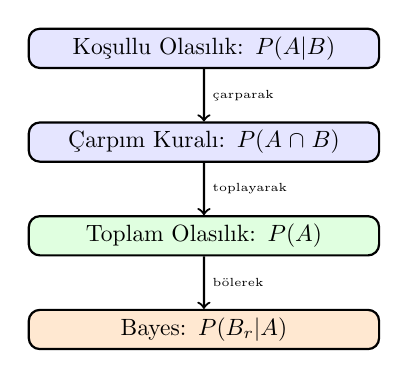
\begin{tikzpicture}[node distance=1.4cm, auto, thick, scale=0.85, transform shape]
                \node (P1) [draw, rounded corners, fill=blue!10, text width=5cm, align=center]
                {Koşullu Olasılık: \(P(A|B)\)};
                \node (P2) [draw, rounded corners, fill=blue!10, below of=P1, text width=5cm, align=center]
                {Çarpım Kuralı: \(P(A\cap B)\)};
                \node (P3) [draw, rounded corners, fill=green!12, below of=P2, text width=5cm, align=center]
                {Toplam Olasılık: \(P(A)\)};
                \node (P4) [draw, rounded corners, fill=orange!18, below of=P3, text width=5cm, align=center]
                {Bayes: \(P(B_r|A)\)};

                \draw[->] (P1) -- (P2) node[midway,right,font=\tiny] {çarparak};
                \draw[->] (P2) -- (P3) node[midway,right,font=\tiny] {toplayarak};
                \draw[->] (P3) -- (P4) node[midway,right,font=\tiny] {bölerek};
            \end{tikzpicture}
            \end{center}
        \end{column}
        \begin{column}{0.48\textwidth}
            \small
            \textbf{Okların anlamı + bağımsızlık yeri:}
            \begin{enumerate}
                \item Koşullu olasılıktan \textbf{çarpım} ile kesişimi buluruz.
                \item \textbf{Bağımsızlık} varsa 1. adım sadeleşir: \(P(A\cap B)=P(A)P(B)\).
                \item \textbf{Tam bağımsızlıkta} 3+ olay için tüm alt kümelerde çarpım kuralı gerekir.
                \item Kesişimleri \textbf{toplayarak} genel $P(A)$'yı elde ederiz.
                \item $P(A)$'ya \textbf{bölerek} gözlemden kaynağa geri döneriz (Bayes).
            \end{enumerate}

            \vspace{0.3cm}
            \textit{Her adım bir öncekinin sonucunu kullanır.}
        \end{column}
    \end{columns}
\end{frame}

\begin{frame}{Hangi Soruda Hangi Yöntem?}
    \begin{block}{Hızlı karar listesi}
        \begin{enumerate}
            \item ``A ve B birlikte/ardışık'' \(\Rightarrow\) Çarpım kuralı
            \item ``X'in genel olasılığı'' ve çoklu senaryo \(\Rightarrow\) Toplam Olasılık
            \item ``X gözlendi, kaynak ne?'' \(\Rightarrow\) Bayes
            \item ``Bağımsız mı?'' \(\Rightarrow\) \(P(A\cap B)\) ile \(P(A)P(B)\) kıyasla
        \end{enumerate}
    \end{block}
\end{frame}

\begin{frame}[fragile]{Mini-Quiz: Yöntemi Tanı}
    \begin{itemize}[<+->]
        \item ``Hem kırmızı hem kusurlu olma olasılığı?'' \(\Rightarrow\) Kesişim/Çarpım
        \item ``Kusurlu olasılığını üç hattan birleştir?'' \(\Rightarrow\) Toplam Olasılık
        \item ``Kusurlu olduğu bilinen ürün hangi hattan geldi?'' \(\Rightarrow\) Bayes
        \item ``Ayrık iki olay bağımsız olabilir mi?'' \(\Rightarrow\) Pozitif olasılıkta hayır
    \end{itemize}
\end{frame}

\begin{frame}{Çıkış Bileti: Evde Kendini Kontrol Et}
    \begin{block}{3 kısa soru}
        \begin{enumerate}
            \item Soruda partition seçimini açıkça gösterebiliyor musun?
            \item \(P(A|B)\) ile \(P(B|A)\) farkını örnekle anlatabiliyor musun?
            \item Sonucun gerçek hayatta makul olup olmadığını test ediyor musun?
        \end{enumerate}
    \end{block}
\end{frame}

\section{Kaynaklar}
\begin{frame}[allowframebreaks]{Kaynaklar}
    \nocite{*}
    \printbibliography{}
\end{frame}

\appendix
\section{Ek: Yapay Zeka Asistanı}
\begin{frame}{Yapay Zeka Asistanınız: NotebookLM}
    \begin{columns}[T]
        \begin{column}{0.48\textwidth}
            \justifying{}
            \textbf{Ders Materyalleri ile Etkileşime Geçin!}
            
            Bu dersin tüm içeriği (sunumlar, makaleler ve notlar), Google'ın gelişmiş yapay zeka asistanı \textbf{NotebookLM} sistemine yüklenmiştir.
            
            \vspace{1em}
            \begin{itemize}
                \item \textbf{Anında Cevaplar:} Aklınıza takılanları sorun.
                \item \textbf{Özetler:} Karmaşık konuları basitçe öğrenin.
                \item \textbf{Audio Overview:} Dersi bir podcast gibi dinleyin.
            \end{itemize}
            
            \vspace{1.5em}
            \begin{center}
                {\setbeamercolor{button}{bg=red,fg=black}
                \href{https://notebooklm.google.com/notebook/2877371a-cb71-4895-90cc-3cb61434962b}{\beamerbutton{\rule[-4ex]{0pt}{11ex}\Large \textbf{Hemen Deneyin}}}}
            \end{center}
        \end{column}
        
        \begin{column}{0.48\textwidth}
            \centering
            \includegraphics[width=\textwidth, height=0.6\textheight, keepaspectratio]{figures/notebooklm.jpg}
        \end{column}
    \end{columns}
\end{frame}

\begin{frame}[plain,noframenumbering]
    \begin{tikzpicture}[remember picture,overlay]
        \node[anchor=center, at=(current page.center), inner sep=0pt] {
            \includegraphics[width=\paperwidth, height=\paperheight]{figures/combined_qrs.png}
        };
        \node[anchor=south, at=(current page.south), yshift=0.5cm, fill=white!95, rounded corners, inner sep=10pt, text width=0.95\paperwidth, align=center] {
            \Large \textbf{\textcolor{blue}{Bizi Takip Edin!}} \\
            \vspace{0.3em}
            \small Ders tekrarlarıyla konuları pekiştirmek (YouTube), profesyonel proje ağlarına katılmak (LinkedIn) ve kampüs duyurularından anında haberdar olmak (Instagram) için topluluğumuza katılın.
        };
    \end{tikzpicture}
\end{frame}

\end{document}
